\documentclass[slidestop]{beamer}
\usepackage{beamerthemesplit}
\usepackage{graphics}
\usepackage{pstricks}

\graphicspath{{./}}

\title{The Libre-SOC Hybrid 3D CPU}
\author{Luke Kenneth Casson Leighton}


\begin{document}

\frame{
   \begin{center}
    \huge{The Libre-SOC Hybrid 3D CPU}\\
    \vspace{32pt}
    \Large{Draft SVP64 in-place Matrix Multiply}\\
    \Large{and FFT / DCT for the Power ISA}\\
    \vspace{24pt}
    \Large{OpenPOWER Summit 2021}\\
    \vspace{16pt}
    \large{Sponsored by NLnet's PET Programme}\\
    \vspace{6pt}
    \large{28th Oct 2021}
  \end{center}
}


\frame{\frametitle{}

\vspace{15pt}

 \begin{itemize}
   \item \vspace{15pt}
   \item \vspace{15pt}
   \item \vspace{15pt}
  \end{itemize}
}

\frame{\frametitle{Overview of Libre-SOC goals}

\vspace{15pt}

 \begin{itemize}
   \item To create power-efficient mass-volume products\vspace{15pt}
   \item To leverage the OpenPOWER ecosystem to do so\vspace{15pt}
   \item To be entirely transparent for Security reasons\vspace{15pt}
   \item To empower businesses to bring Secure transparent\\
         mass-volume products to market\vspace{15pt}
  \end{itemize}
}

\frame{\frametitle{Overview of SVP64 goals}

\vspace{15pt}

 \begin{itemize}
   \item High performance and high performance/watt\vspace{15pt}
   \item Reduced code density (reduced I-Cache usage)\\
         https://arxiv.org/abs/2002.10143 - 3.5x power reduction\vspace{8pt}
   \item Remain accessible for assembler writers and compilers alike\vspace{15pt}
   \item Introduce true Vectorisation to the Power ISA\\
         (VSX is Packed SIMD)\vspace{8pt}
   \item Be adopted via the external OPF ISA WG RFC process\\
         (not: be a non-official custom extension. proprietary\\
         custom extensions conflict with mass-volume adoption)\vspace{15pt}
  \end{itemize}
}



%%\frame{\frametitle{nmigen PowerISA Decoder}

%%\begin{center}
%%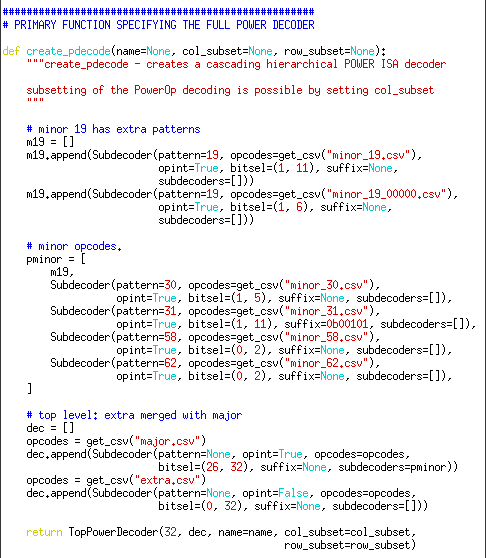
\includegraphics[width=0.55\textwidth]{2020-09-09_21-04.png}
%%\end{center}

%%}

\begin{frame}[fragile]
\frametitle{Reminder of Simple-V}

\begin{semiverbatim}
https://libre-soc.org/openpower/sv/overview/
Greatly simplified (like x86 "REP" instruction):

  for (i = 0; i < VL; i++)
       GPR[RT+i] <= GPR[RA+i] + GPR[RB+i];

function op\_add(RT, RA, RB, predr) # add not VADD!
  int i, id=0, irs1=0, irs2=0;
  for (i = 0; i < VL; i++)
    if (GPR[predr] & 1<<i) # predication
       GPR[RT+id] <= GPR[RA+irs1] + GPR[RB+irs2];
    if (reg\_is\_vectorised[RT])  \{ id += 1; \}
    if (reg\_is\_vectorised[RA])  \{ irs1 += 1; \}
    if (reg\_is\_vectorised[RB])  \{ irs2 += 1; \}
\end{semiverbatim}

\end{frame}


\begin{frame}[fragile]
\frametitle{SVP64 REMAP system}

\begin{semiverbatim}
Register offsets are "REMAP"ed through a Hardware FSM
https://libre-soc.org/openpower/sv/remap/
remarkably similar to ZOLC
https://www.researchgate.net/publication/224647569

function op\_add(RT, RA, rs2, predr) # add not VADD!
  int i, id=0, irs1=0, irs2=0;
  for (i = 0; i < VL; i++)
    if (GPR[predr] & 1<<i) # predication
       GPR[RT+REMAP(id)] <= GPR[RA+REMAP(irs1)] +
                           GPR[rs2+REMAP(irs2)];
    if (reg\_is\_vectorised[RT])  \{ id += 1; \}
    if (reg\_is\_vectorised[RA])  \{ irs1 += 1; \}
    if (reg\_is\_vectorised[s2])  \{ irs2 += 1; \}
\end{semiverbatim}

\end{frame}

\begin{frame}[fragile]
\frametitle{Matrix Multiply: Basics}

\begin{semiverbatim}
(a00 a01 a02  x (b00 b01   =
 a10 a11 a12)    b10 b11
                 b20 b21)

(a00*b00 + a01*b10 + a02*b20 a00*b01 + a01*b11 + a02*b21
 a10*b00 + a11*b10 + a12*b20 a10*b01 + a11*b11 + a12*b21)

 (b00 b01    x (a00 a01 a02  =
  b10 b11       a10 a11 a12)
  b20 b21)

(b00*a00 + b01*a10  b00*a01 + b01*a11  b00*a02 + b01*a12
 b10*a00 + b11*a10  b10*a01 + b11*a11  b10*a02 + b11*a12
 b20*a00 + b21*a10  b20*a01 + b21*a11  b20*a02 + b21*a12)

\end{semiverbatim}

\end{frame}


\begin{frame}[fragile]
\frametitle{Matrix Multiply: naive, with python for-loops}

\begin{semiverbatim}
result = [] # final result
for i in range(len(A)):

  row = [] # the new row in new matrix
  for j in range(len(B[0])):

    product = 0 # the new element in the new row
    for v in range(len(A[i])):
        product += A[i][v] * B[v][j]
    row.append(product) # add sum of product to new row

  result.append(row) # add new row into final result
\end{semiverbatim}

\end{frame}

\begin{frame}[fragile]
\frametitle{Matrix Multiply: suitable for Hardware scheduling}

\begin{semiverbatim}
Unsuitable: creates massive Read-After-Write chains

for i in range(len(A)):
  for j in range(len(B[0])):
    for v in range(len(A[i])):
      product[i][j] += A[i][v] * B[v][j]

Suitable: can be parallelised / pipelined. RaW avoided

for i in range(len(A)):
  for v in range(len(A[i])):    # swapped
    for j in range(len(B[0])):  # with this
      product[i][j] += A[i][v] * B[v][j]

\end{semiverbatim}

\end{frame}


\frame{\frametitle{Matrix Multiply: Generalise but Specialise}

\vspace{8pt}

 \begin{itemize}
   \item Why not make a general-purpose nested "Loop" system?\\
        - Other uses (algorithms) beyond Matrix Multiplication\\
        - Allow any arbitrary-sized loops\\
        - Allow any permutation of nesting\\
        - Allow reversing per-dimension\vspace{5pt}
   \item Specialise by making Matrix Multiply "setup" quick/easy\\
        - two 32-bit instructions to set up A, B, C sizes\\
        - one 64-bit SVP64 FMAC instruction.\\
        - Nothing else needed.  Saves on I-Cache\vspace{5pt}
   \item Hardware turns out to be near-identical to ZOLC\\
        https://opencores.org/projects/hwlu\\
        https://libre-soc.org/openpower/sv/remap/\vspace{15pt}
  \end{itemize}
}

\begin{frame}[fragile]
\frametitle{Matrix Multiply: unit test / example}

\begin{semiverbatim}
  94 def test_sv_remap2(self):
  95     lst = ["svshape 5, 4, 3, 0, 0",
  96            "svremap 0b11111, 1, 2, 3, 0, 0, 0, 0",
  97            "sv.fmadds 0.v, 8.v, 16.v, 0.v"
  98           ]
  99             REMAP fmadds FRT, FRA, FRC, FRB

svshape 5, 4, 3, 0, 0 => A: 3x5 B: 3x4
                      => C: 3x3
svremap (enable) (F)RS, (F)RT, (F)RA, (F)RB, (F)RC
sv.fmadds: uses fp0 as accumulator
      product[i][j] += A[i][v] * B[v][j]
\end{semiverbatim}

\end{frame}

\frame{\frametitle{Matrix Multiply: Ehm that's all Folks}

\vspace{6pt}

 \begin{itemize}
   \item Really is that straightforward: no actual Vector ops\\
        - Does not dictate or limit micro-architectural detail\\
        - Issues Scalar FMACs into existing back-end hardware\\
        - Can use any 4-operand instruction (GF, INT, Bitmanip)\\
        - No Power-2 limits. Any operand width (8/16/32/64)\vspace{8pt}
   \item Limited to 127 scalar ops and in-place registers.  Future?\\
        - https://arxiv.org/abs/2002.10143 CISC-like load-and-inc\\
        - Auto-load/store (tagged) registers, keeps RISC ISA\\
        - Extend to memory-based arbitrary NxN matrix sizes\\
        - Still power-efficient: no I-cache usage during FMAC issue\vspace{8pt}
   \item Future can be investigated as part of EUR 22.6m EU Grant\\
        https://libre-soc.org/SEP-210803722-Libre-SOC-8-core/\vspace{15pt}
  \end{itemize}
}


\frame{\frametitle{TODO rewrite Summary}

 \begin{itemize}
   \item Goal is to create a mass-volume low-power embedded SoC suitable
         for use in netbooks, chromebooks, tablets, smartphones, IoT SBCs.
   \item No DRM. 'Trustable' (by the users, not by Media Moguls) design
         ethos as a \textit{business} objective: requires full transparency
         as well as Formal Correctness Proofs
   \item Collaboration with OpenPOWER Foundation and Members absolutely
         essential. No short-cuts.  Standards to be developed and ratified
         so that everyone benefits.
   \item Working on the back of huge stability of POWER ecosystem
   \item Combination of which is that Board Support Package is 100\%
         upstream, app and product development by customer is hugely
         simplified and much more attractive

  \end{itemize}
}


\frame{
  \begin{center}
    {\Huge The end\vspace{15pt}\\
		   Thank you\vspace{15pt}\\
		   Questions?\vspace{15pt}
	}
  \end{center}

  \begin{itemize}
	\item Discussion: Libre-SOC-dev mailing list
	\item Freenode IRC \#libre-soc
	\item http://libre-soc.org/
	\item http://nlnet.nl/PET
  \end{itemize}
}


\end{document}
